\documentclass{article}
%%%%%%%%%%%%%
% Loads packages
%%%%%%%%%%%%%
\usepackage[table]{xcolor}
\usepackage[utf8]{inputenc}
\usepackage[colorlinks=true,linkcolor=blue]{hyperref}
\usepackage{geometry} %package needed to set margins
\usepackage{fancyhdr}
\usepackage{graphicx}
\usepackage{amsmath}
\usepackage{amsthm}
\usepackage{mdframed}
\usepackage{tikz}
\usetikzlibrary{arrows.meta}
\usetikzlibrary{decorations.markings}
\usepackage{amsfonts}
\usepackage{wasysym}
\usepackage{listings}% http://ctan.org/pkg/listings
\lstset{
basicstyle=\ttfamily,
mathescape
}
\pagestyle{fancy}
\fancyhf{}
\chead{\textbf{Homework 9}}
\lhead{Math 213, Fall 2024}
\rhead{Due Sunday, 11/10 at 11:59pm}
%%%%%%%%%%%%%
% Sets margins
%%%%%%%%%%%%%
\newgeometry{left=1.5in,right=1in,top=1in,bottom=1in}
\setlength\headsep{3pt}
%%%%%%%%%%%%%
% Creates problem and solution environments
%%%%%%%%%%%%%
% Solution Environment
\newenvironment{solution}{\begin{proof}[Solution]}{\end{proof}}
% Problem Environment
\newenvironment{problem}[1]
{\begin{mdframed}[default]
\textbf{Problem #1:}
}
{\end{mdframed}
}
%%%%%%%%%%%
% Custom Commands
%%%%%%%%%%%
\newcommand{\gOne}{\cellcolor{green!50!white} 1}
\newcommand{\rZero}{\cellcolor{red!50!white} 0}
\begin{document}
\begin{problem}{\S 9.5 - 3(c,d,e)}
Which of these relations on the set of all functions from $\mathbb{Z}$ to $\mathbb{Z}$ are equivalence relations? Determine the properties of an equivalence
relation that the others lack.
\begin{itemize}
\item[(c)] $\{ (f,g)~:~ f(x)-g(x) = 1 \textrm{ for all } x \in \mathbb{Z}\}$.
\item[(d)] $\{ (f,g)~: \textrm{ for some } C \in \mathbb{Z}, \textrm{ for all }
x \in \mathbb{Z}, f(x) - g(x) = C \}$.
\item[(e)] $\{ (f,g)~|~f(0) = g(1) \textrm{ and } f(1) = g(0) \}$.
\end{itemize}
Solution:
\begin{itemize}
    \item[(c)] Since $f(x)-f(x)=0$, it is not reflexive. Since $f(x)-g(x)=1$, $g(x)-f(x)=-1$, so it is not symmetric. Since $f(x)-g(x)=1$, $g(x)-h(x)=1$, $f(x)-h(x)=2$, so not transitive. So not equivalence.
    \item[(d)] Since $f(x)-f(x)=0$, $0\in \mathbb{Z}$, it is reflexive. Since $f(x)-g(x)=C$, take both side negative, $g(x)-f(x)=-C$, $-C\in \mathbb{Z}$, it is symmetric. And 
    Since $f(x)-g(x)=C_1$, $g(x)-h(x)=C_2$, $f(x)-h(x)=f(x)-g(x)+g(x)-h(x)=C_1+C_2=C$, so it is transitive. So, this is equivalence relation.
    \item[(e)] For $f$ to be reflexive, we must have $f(0)=f(1)$. This is not necessarily true for all functions, so not reflexive. Since $f(0)=g(1)$ and $f(1)=g(0)$ is same as $g(0)=f(1)$ and $g(1)=f(0)$, so symmetric. Since $f(0)=g(1)$ and $f(1)=g(0)$, $g(0)=h(1)$ and $g(1)=h(0)$, $f(0)=h(0)$ and $f(1)=h(1)$, so not transitive. So not equivalence.
\end{itemize}
\end{problem}
\begin{problem}{\S 9.5 - 22}
Determine whether the relation with the directed graph shown is an equivalence
relation.
\begin{center}
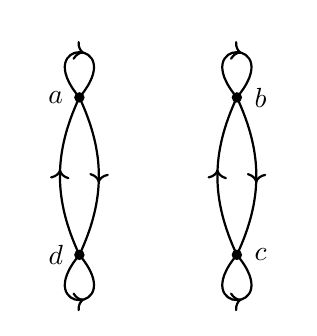
\begin{tikzpicture}
\begin{scope}[thick,decoration={
markings,
mark=at position 0.54 with {\arrow{>}}}
]
% draws vertices
\node[circle, fill=black,scale = 0.4] at (0,0){};
\node[circle, fill=black,scale = 0.4] at (0,2){};
\node[circle, fill=black,scale = 0.4] at (2,2){};
\node[circle, fill=black,scale = 0.4] at (2,0){};
% draws directed edges
\draw[postaction={decorate},out=115,in=-115] (0,0) to (0,2);
\draw[postaction={decorate},out=-65,in=65] (0,2) to (0,0);
\draw[postaction={decorate},out=115,in=-115] (2,0) to (2,2);
\draw[postaction={decorate},out=-65,in=65] (2,2) to (2,0);
\draw[scale=2,postaction={decorate}] (0,0) to[out=-130,in=-50,loop] (0,0);
\draw[scale=2,postaction={decorate}] (1,0) to[out=-130,in=-50,loop] (1,0);
\draw[scale=2,postaction={decorate}] (1,1) to[out=130,in=50,loop] (1,1);
\draw[scale=2,postaction={decorate}] (0,1) to[out=130,in=50,loop] (0,1);
% labels vertices
\node at (-0.3,0) {$d$};
\node at (-0.3,2) {$a$};
\node at (2.3,2) {$b$};
\node at (2.3,0) {$c$};
\end{scope}
\end{tikzpicture}
\end{center}
Solution:
Since every point have an arrow pointing it self, meaning that $(a,a)\in R$, so it is reflexive.
Since every arrow between two points are double arrow, meaning that $(a,d)=(d,a)$, so it is symmetric.
Since all of the length two are accompanied by length one, so it is transitive. So it is equivalence. And equivalence classes are $(a,d)$ and $(b,c)$
\end{problem}
\begin{problem}{\S 9.5 - 24(a,b)}
Determine whether the relations represented by these binary matrices are
equivalence relations.
\begin{itemize}
\item[(a)] $\begin{bmatrix} 1 & 1 & 1 \\ 0 & 1 & 1 \\ 1 & 1 & 1 \end{bmatrix}$
\item[(b)] $\begin{bmatrix} 1 & 0 & 1 & 0 \\ 0 & 1 & 0 & 1 \\ 1 & 0 & 1 & 0 \\
0 & 1 & 0 & 1 \end{bmatrix}$
\end{itemize}
Solution:
\begin{itemize}
    \item[(a)] Since all the diagonal are 1, it is reflexive. Since it is not a symmetric matrix, it is not symmetric relation. So don't need to verify transitive it is already not equivalence.
    \item[(b)] Since all the diagonal are 1, it is reflexive. Since it is symmetric matrix, it is symmetric relation. Since there are no $(i,j)$, $(j,k)$ in R, but $(i,k)\notin R$, it is transitive. So it is equivalence, and equivalence class is $(1,3)$ and $(2,4)$
\end{itemize}
\end{problem}
\begin{problem}{\S 9.5 - 30(a,b)}
What are the equivalence classes of these bit strings for the equivalence relation
\[ R = \{ (x,y)~:~ x \textrm{ and } y \textrm{ are binary strings of length three
or more that agree in the first three bits}\} \]
\begin{itemize}
\item[(a)] 010
\item[(b)] 1011
\end{itemize}
Solution:
\begin{itemize}
    \item[(a)] All bit strings with first three digit of 010
    \item[(b)] All bit strings with first three digit of 101
\end{itemize}
\end{problem}
\begin{problem}{\S 9.5 - 44(a,b,e)}
Which of these collections of subsets are partitions of the set of integers?
\begin{itemize}
\item[(a)] the set of even integers and the set of odd integers.
\item[(b)] the set of positive integers and the set of negative integers.
\item[(e)] the set of integers not divisible by 3, the set of even integers,
and the set of integers that leave a remainder of 3 when divided by 6.
\end{itemize}
Solution:
\begin{itemize}
    \item[(a)]The set of even integers and the set of odd integers are disjoint and non-empty, also, add up together is the whole set of integers. So, they are partitions of set of integers.
    \item[(b)]The set of positive integers and set of negative integers are disjoint and non-empty. But 0 is in neither set. So, they are NOT partitions of set of integers.
    \item[(c)]The integers not divisible by 3 include the integers divisible by two, which is even integers, so they are not disjoint, then they are not partitions of set of integers.
\end{itemize}

\end{problem}
\begin{problem}{\S 9.5 - 48(a)}
List the ordered pairs in the equivalence relation produced by the following
partition of $\{ a, b, c, d, e, f, g \}$:
\[ \{ a, b \}, \{ c, d \}, \{ e, f, g \} \]

Solution:

$\{(a,a),(b,b),(c,c),(d,d),(e,e),(f,f),(g,g),(a,b),(b,a),$

$(c,d),(d,c),(e,f),(f,e),(e,g),(g,e),(f,g),(g,f)\}$
\end{problem}
\begin{problem}{\S 10.1 - 28}
Describe a graph model that represents a subway system in a large city. Should
edges be directed or undirected? Should multiple edges be allowed? Should loops be
allowed?

Solution:

For a subway graph, edge should be directed since suppose there exist one way segment , every line have a direction to go (If does not exist one way segment, than can be undirected). And should multiple edges be allowed, since sometime there will be two different line between two stations. And loops should not be allowed too, since no one will take a train to its original station.
\end{problem}
\begin{problem}{\S 10.2 - 8}
Determine the number of vertices and edges and find the in-degree and out-degree of
each vertex for the following graph:
\begin{center}
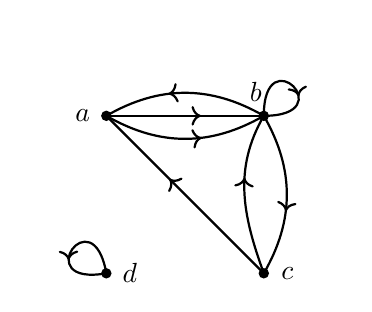
\begin{tikzpicture}
\begin{scope}[thick,decoration={
markings,
mark=at position 0.6 with {\arrow{>}}}
]
% draws vertices
\node[circle, fill=black,scale = 0.4] at (0,0){};
\node[circle, fill=black,scale = 0.4] at (2,0){};
\node[circle, fill=black,scale = 0.4] at (0,2){};
\node[circle, fill=black,scale = 0.4] at (2,2){};
% labels vertices
\node at (-0.3,2) {$a$};
\node at (1.9,2.3) {$b$};
\node at (2.3,0) {$c$};
\node at (0.3,0) {$d$};
% draws edges
\draw[postaction={decorate}] (2,0) to (0,2);
\draw[postaction={decorate}] (0,2) to (2,2);
\draw[postaction={decorate},out=-30,in=210] (0,2) to (2,2);
\draw[postaction={decorate},out=150,in=30] (2,2) to (0,2);
\draw[postaction={decorate},out=-60,in=60] (2,2) to (2,0);
\draw[postaction={decorate},out=110,in=240] (2,0) to (2,2);
% draws loops
\draw[scale=2,postaction={decorate}] (0,0) to[out=100, in=190,loop]
(0,0);
\draw[scale=2,postaction={decorate}] (1,1) to[out=90, in=0,loop] (1,1);
\end{scope}
\end{tikzpicture}
\end{center}
Solution:

There are 4 vertices and 8 edges. 

Vertex $a$ has in-degree of 2 and out-degree of 2. 

Vertex $b$ has in-degree of 4 and out-degree of 3.

Vertex $c$ has in-degree of 1 and out-degree of 2. 

Vertex $d$ has in-degree of 1 and out-degree of 1. 
\end{problem}
\begin{problem}{\S 10.2 - 10}
For the graph in Problem $\S 10.2 - 8$, determine the sum of the in-degrees of the
vertices and the sum of the out-degree of the vertices directly. Show that they are
both equal to the number of edges in the graph.

Solution:

The sum of in-degree of vertices: $2+4+1+1=8$

The sum of out-degree of vertices: $2+3+2+1=8$

Since $8=8$, and after calculation, there are 8 edges in total in the graph. so they are both equal to the number of edges in the graph.
\end{problem}
\begin{problem}{\S 10.2 - 35(a,b,c)}
How many vertices and how many edges do these graphs have?
\begin{itemize}
\item[(a)] $K_n$.
\item[(b)] $C_n$.
\item[(c)] $W_n$.
\end{itemize}

Solution:

\begin{itemize}
    \item[(a)] Since $K_n$ meaning that every two vertices are connected by unique edge. So there are $n$ vertices, and number of edge is ${n \choose 2}=\frac{n!}{(n-2)!2!}$.
    \item[(b)] Since $C_n$ Form a single cycle where each vertex is connected to exactly two other vertices. There are $n$ vertices, since a single cycle formed, there are $n$ edges.
    \item[(c)] Since $W_n$ is Consists of a cycle $C_{n}$ with an additional central hub vertex connected to all peripheral vertices. So there are $n+1$ vertices, and there will be $2n$ edges since there are a cycle for $n$ vertices and a vertex connected to all those $n$ vertices.
\end{itemize}
\end{problem}
\begin{problem}{\S 10.2 - 37(a,b,c)}
Find the degree sequence of each of the following graphs.
\begin{itemize}
\item[(a)] $K_4$.
\item[(b)] $C_4$.
\item[(c)] $W_4$.
\end{itemize}
Solution:

\begin{itemize}
    \item[(a)] Since each two vertices are connected except loop to itself, and 4 vertices as a whole, the degree sequence is $[3,3,3,3]$
    \item[(b)] Since there are a cycle formed, every vertices are only connected to two other vertices, and there are 4 vertices in total, the degree sequence is $[2,2,2,2]$
    \item[(c)] Since there are a cycle formed, and there are another one vertices connected to every vertices. So, the sequence should be $[3,3,3,3,4]$
\end{itemize}
\end{problem}
\end{document}